\section{Giới thiệu đề tài}
\subsection{Thực trạng}
\subsubsection{Thực trạng chung}
\indent \indent Trong bối cảnh xã hội hiện nay, cùng với sự phát triển mạnh mẽ của Internet và các nền tảng thương mại điện tử, việc mua vé sự kiện trực tuyến đang trở thành xu hướng phổ biến. Người dùng có thể dễ dàng tham gia các chương trình ca nhạc, hội nghị, lễ hội hoặc workshop chỉ với vài thao tác trên trình duyệt.\\
\indent Theo báo cáo của The Business Research Company (2024), quy mô thị trường đặt vé sự kiện trực tuyến toàn cầu đạt 50,97 tỷ USD vào năm 2024 và dự kiến sẽ tăng lên 67,89 tỷ USD vào năm 2029, với tốc độ tăng trưởng trung bình (CAGR) 6,4\%/năm.\\
\indent Tại Việt Nam, theo 6W Research (2025), thị trường đặt vé sự kiện trực tuyến được dự báo tăng trưởng mạnh mẽ trong giai đoạn 2025–2031, nhờ sự phát triển của hạ tầng thanh toán điện tử và tỷ lệ người dùng Internet cao. \\
\indent Với những lợi ích thiết thực đó, hình thức đặt vé sự kiện trực tuyến ngày càng được hệ thống rộng rãi trong nhiều lĩnh vực khác nhau. Chẳng hạn, trong ngành giải trí, các nền tảng đặt vé hỗ trợ người dùng mua vé concert, phim, lễ hội chỉ với vài thao tác trên trình duyệt; trong giáo dục, các trường học có thể áp dụng hệ thống để tổ chức và quản lý các sự kiện lớn như Job Fair, cuộc thi học thuật, hội nghị hay đại hội,... thay vì sử dụng các biểu mẫu đăng ký truyền thống. \\
\indent Việc số hóa quy trình bán vé không chỉ mang lại trải nghiệm thuận tiện và minh bạch cho người dùng, mà còn giúp Ban tổ chức tiết kiệm thời gian, giảm chi phí nhân sự và kiểm soát tốt hơn doanh thu cũng như lượng người tham dự.\\
% \indent Nhóm thực hiện đã tiến hành một khảo sát nhỏ trong các hội nhóm mạng xã hội dành cho người thường xuyên tham gia sự kiện, kết quả thu được:
% \begin{itemize}
%     \item[-] 86\% người được hỏi cho rằng họ ưu tiên mua vé online thay vì mua tại quầy.
%     \item[-] 31\% cho rằng các nền tảng hiện tại khó thao tác hoặc giao diện chưa thân thiện.
%     \item[-] 78\% nói rằng liên hệ với Ban tổ chức để được hỗ trợ còn nhiều khó khăn.
%     \item[-] 62\% mong muốn có chức năng đánh giá và phản hồi sau sự kiện.
% \end{itemize}
% \begin{figure}[H]
%     \centering
%     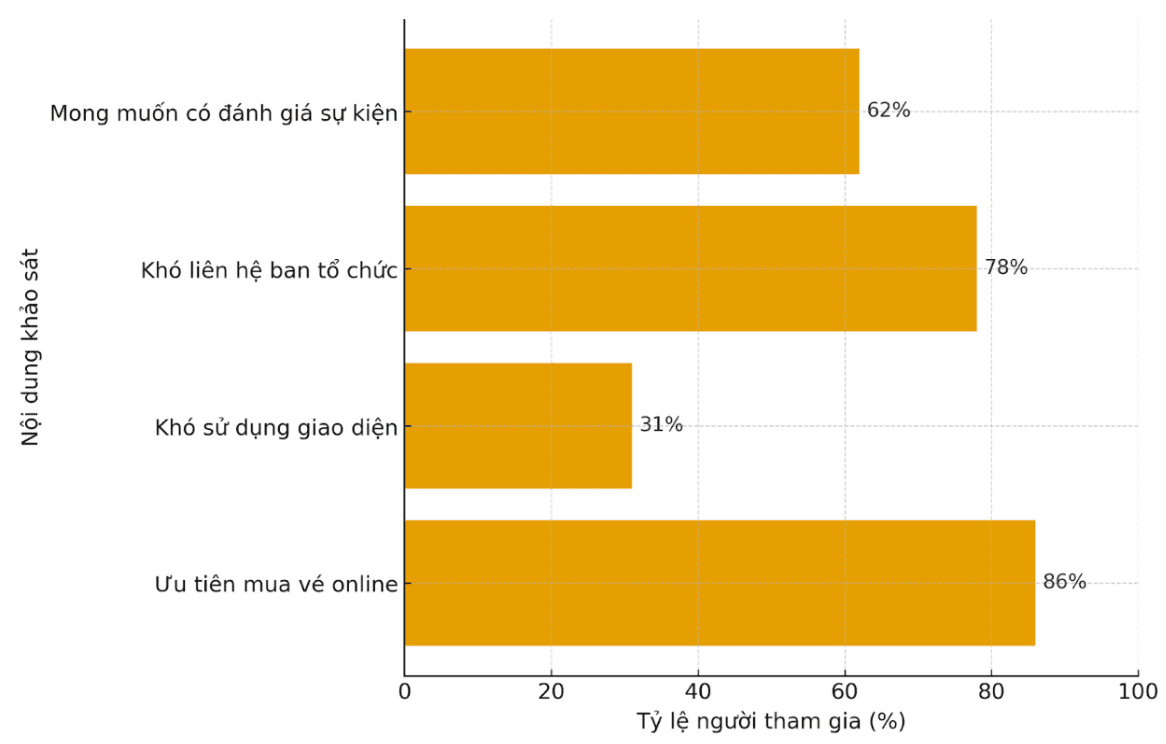
\includegraphics[width=0.7\textwidth]{Images/KhaoSat.png}
%     \vspace{10pt}
%     \caption{Kết quả khảo sát dành cho người tham gia sự kiện}
%     \label{fig:khao_sat}
% \end{figure}
% \indent \indent Các kết quả này cho thấy nhu cầu có một nền tảng đặt vé sự kiện đơn giản, tiện lợi, bảo mật và có tính tương tác cao là vô cùng cần thiết, đặc biệt trong bối cảnh Việt Nam đang đẩy mạnh chuyển đổi số trong lĩnh vực giải trí và dịch vụ.
\subsubsection{Thực trạng các hệ thống hiện có}
\indent \indent Với sức hút ngày càng lớn của các sự kiện cùng sự tiện lợi mà các công nghệ mang lại, tại Việt Nam nhiều nền tảng cung cấp dịch vụ đặt vé trực tuyến đã ra đời. 
Để đánh giá thực trạng các hệ thống này, nhóm đã tiến hành khảo sát và phân tích ba nền tảng phổ biến bao gồm TicketBox, VnTicket và Ticketgo dựa trên các tiêu chí về tính tiện dụng, hệ thống gợi ý và khả năng hỗ trợ tự động. 
Kết quả như sau:

\begin{table}[H]
\centering
\renewcommand{\arraystretch}{1.3}
\setlength{\tabcolsep}{6pt}
\begin{tabularx}{\textwidth}{|l|X|X|X|}
\hline
\textbf{Nền tảng} & \textbf{Tính tiện dụng} & \textbf{Hệ thống gợi ý} & \textbf{Khả năng hỗ trợ tự động} \\ \hline

\textbf{TicketBox} 
& Giao diện hiện đại, UX/UI thân thiện; tích hợp thanh toán (Momo, ngân hàng); quy trình đặt vé nhanh, nhận E-ticket tiện lợi 
& Gợi ý ở mức cơ bản, chủ yếu dựa trên xu hướng (Trending), chưa cá nhân hóa sâu 
& Hỗ trợ ở mức trung bình, chưa có hệ thống phản hồi tự động thông minh \\ \hline

\textbf{VnTicket} 
& Độ uy tín cao; phù hợp sự kiện lớn (thể thao, nghệ thuật); tuy nhiên giao diện và công nghệ còn cũ 
& Hầu như chưa có hệ thống gợi ý thông minh, ít cá nhân hóa 
& Hỗ trợ chậm khi có lỗi; thiếu hệ thống tự động hóa \\ \hline

\textbf{Ticketgo} 
& Dễ sử dụng cho sự kiện vừa và nhỏ; quy trình tạo và quản lý sự kiện đơn giản 
& Gợi ý hạn chế do quy mô dữ liệu nhỏ; chưa phát triển cá nhân hóa 
& Chủ yếu hỗ trợ qua hotline/chat thủ công; chưa tích hợp chatbot tự động \\ \hline

\end{tabularx}
\vspace{15pt}
\caption{So sánh các nền tảng đặt vé tại Việt Nam theo tính năng chính}
\label{tab:so_sanh_he_thong_ve}
\end{table}

Thông qua bảng so sánh trên, nhóm nhận thấy các hệ thống trên vẫn vận hành theo mô hình truyền thống—chủ yếu tập trung vào việc hoàn thiện luồng nghiệp vụ mua/bán thuần túy—mà chưa chú trọng đúng mức vào việc tối ưu hóa trải nghiệm tương tác thông minh cho người dùng.
Qua đó, nhóm rút ra một số nhận định quan trọng làm cơ sở cho việc phát triển đề tài:
\begin{itemize}
    \item[1.] Sự thiếu hụt về tính tương tác: Các hệ thống hiện nay mang tính chất "tĩnh", người dùng phải chủ động tìm kiếm qua các bộ lọc thủ công. Việc thiếu vắng một giao diện hội thoại thông minh (Conversational AI) khiến quy trình tư vấn và giải đáp thắc mắc thường bị gián đoạn.
    \item[2.] Hệ thống gợi ý chưa sâu: Việc đề xuất sự kiện thường dựa trên số đông thay vì phân tích dữ liệu lịch sử và sở thích thực tế của từng cá nhân.
    \item[3.] Áp lực hỗ trợ khách hàng: Việc phụ thuộc vào hotline hoặc nhân sự trực chat truyền thống tạo ra độ trễ lớn khi số lượng yêu cầu tăng đột biến, đồng thời không đảm bảo khả năng hỗ trợ 24/7.
\end{itemize}

\subsection{Mục tiêu và Phạm vi đề tài}
\indent \indent Dựa trên việc phân tích những hạn chế của thực trạng, đề tài hướng tới xây dựng một hệ thống không chỉ giải quyết bài toán đặt vé mà còn đóng vai trò một "trợ lý sự kiện" thông minh.\\
\indent \textbf{Về mục tiêu đề tài}: Nhóm đặt ra các mục tiêu cụ thể như sau:
\begin{itemize}
\item[1.] Xây dựng nền tảng đặt vé hiện đại, tối ưu hóa quy trình thanh toán qua cổng PayOS.
\item[2.] Ứng dụng thuật toán học máy (Machine Learning) để cá nhân hóa trải nghiệm người dùng thông qua hệ thống gợi ý.
\item[3.] Tích hợp Chatbot AI để hỗ trợ 24/7, giải quyết triệt để vấn đề "nghẽn" hỗ trợ khách hàng.
\end{itemize}

\indent \textbf{Về phạm vi đề tài}: Để đảm bảo tính khả thi và tập trung vào các vấn đề cốt lõi, nhóm sẽ giới hạn phạm vi nghiên cứu và phát triển như sau:
\begin{itemize}
\item[1.] \textbf{Nền tảng:} Tập trung phát triển phiên bản Web (Responsive) để đảm bảo tính ổn định và tiếp cận nhanh.
\item[2.] \textbf{Thanh toán:} Hỗ trợ phương thức thanh toán chuyển khoản nhanh qua cổng PayOS.
\item[3.] \textbf{Công nghệ cốt lõi:}
\begin{enumerate}
\item[-] Hệ thống đặt vé trực tuyến (Web Booking).
\item[-] Hệ thống gợi ý (Recommendation System) dựa trên lịch sử tương tác.
\item[-] Chatbot AI (Conversational AI) hiểu ngôn ngữ tự nhiên để tư vấn sự kiện.
\end{enumerate}
\end{itemize}
